\subsection{UWSpine dataset\label{sec:UWspine}}
 
This dataset is made available by the Department of Radiology of the University of Washington\footnote{Creative Commons Attribution-NonCommercial-NoDerivatives 4.0 International License, dataset available at \url{
      https://biomedia.doc.ic.ac.uk/data/spine/  
    }}.
It has been constructed by dr. Glocker and team \cite{Glocker2012,Glocker2013} (Microsoft research) in 2012.
For each scan, manual annotations of vertebrae centroids are provided.
This dataset contains 242 \acrshort{ct} scans of 150 different patients.
This dataset does not contain full mask labels, only centroid point annotations.
To investigate the relative performance of a weakly supervised model compared to the performance of a fully supervised model, both will be trained on the same dataset\footnote{The modelling concept is further discussed in chapter \ref{sec:model_concept}.}.
Furthermore, the evaluation of the models is based on the full annotations.
Thus, the UWSpine dataset will not be used for model training.
It will only be used for visual evaluation of the model on an entirely new dataset\footnote{The UWSpine dataset is \textit{completely} new in the sense that no samples from this dataset (this \textit{population}, so to speak) are present in the train or validation set.
For the \textit{regular} test set, other samples from the same datasets were present in the train and validation sets.}.


\subsubsection{Original Objective of the Dataset}

In \cite{Glocker2012,Glocker2013} the development of a model based on regression forests and a \acrfull{hmm} for vertebra localisation without needing strong assumptions on what part of the spine is visible.

\subsubsection{Patient statistics}


Figure \ref{fig:UW_ageboxplot} illustrated that the patients in the \textit{UWSpine} dataset are relatively varied in age.
Of most patients in the dataset, multiple scan images are available.
The highest number of scans taken from a single patient is 5.

\subsubsection{Technical information}

Only volume centre point annotations are available for the \textit{UWSpine} dataset. 
This dataset is thus annotated even more sparsely than what is considered as weak supervision in this work.
Instead of providing an annotation point per slice, one annotation point per vertebra volume is provided and not annotation points for the background class.

The scans in the \textit{UWSpine} dataset are strongly cropped around the spine, both in the left-right direction and the anteroposterior direction.

\begin{SCfigure}[][htb]
    \centering
    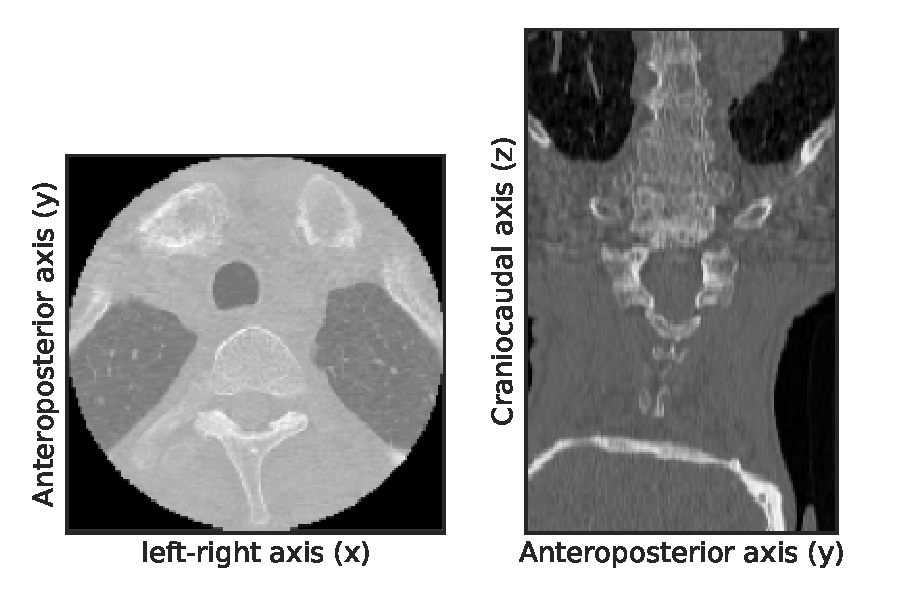
\includegraphics[width=.95\textwidth]{automated_graphs/UW_4564688.pdf}
    \caption{University of Washington dataset, scan \textit{4564688}. \label{fig:UW_4564688}}
\end{SCfigure}

\marginpar{
        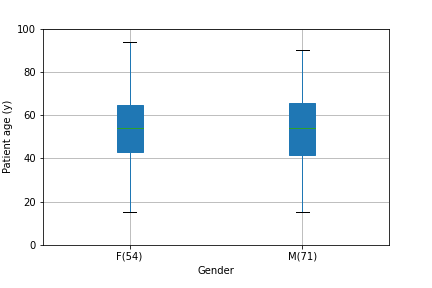
\includegraphics[width=5cm]{automated_graphs/UW_ageboxplot.png}
        \captionof{figure}{Distribution of patient age in the dataset from Washington University.}
        \label{fig:UW_ageboxplot}
    }